\section{Các linh kiện chính}
\renewcommand{\arraystretch}{1.5} % Tăng khoảng cách giữa các dòng
\begin{center}
\begin{tabular}{|c|c|c|>{\centering\arraybackslash}m{3cm}|}
    \hline
    \textbf{STT} & \textbf{Tên linh kiện} & \textbf{Số lượng} & \textbf{Hình ảnh} \\
    \hline
    1 & PIC16F887 & 1 & 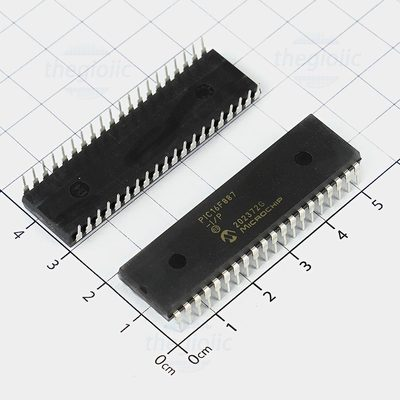
\includegraphics[width=2.5cm]{pictures/pic16f887.png} \\
    \hline
    2 & Đế ra chân PIC & 1 & 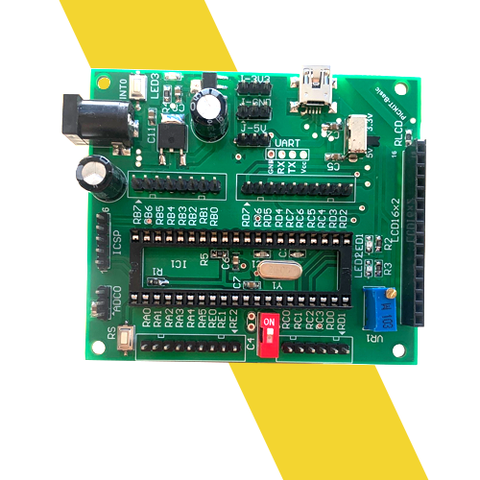
\includegraphics[width=2.5cm]{pictures/kitpic.png} \\
    \hline
    3 & Mạch đèn giao thông & 4 & 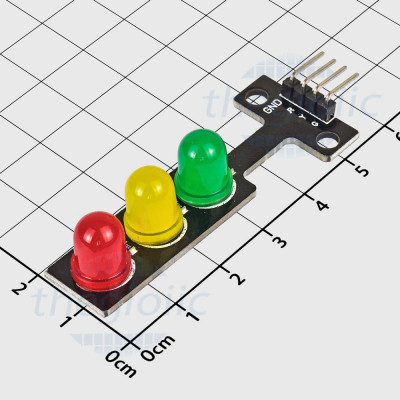
\includegraphics[width=2.5cm]{pictures/traficlight.png} \\
    \hline
    4 & Module 2 LED 7 đoạn 74HC595  & 4 & 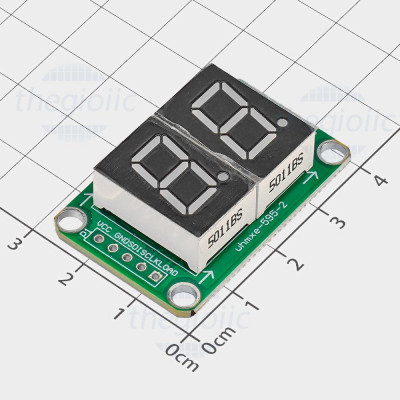
\includegraphics[width=2.5cm]{pictures/7led.png} \\
    \hline
    5 & LCD 1602 & 1 & 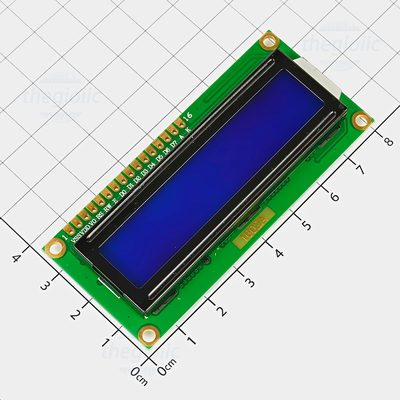
\includegraphics[width=2.5cm]{pictures/lcd.png} \\
    \hline
    6 & Mạch giao tiếp LCD I2C & 1 & 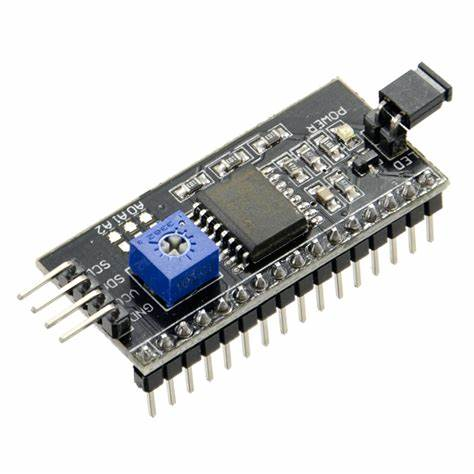
\includegraphics[width=2.5cm]{pictures/i2c.png} \\
    \hline
    7 & Nút nhấn & 3 & 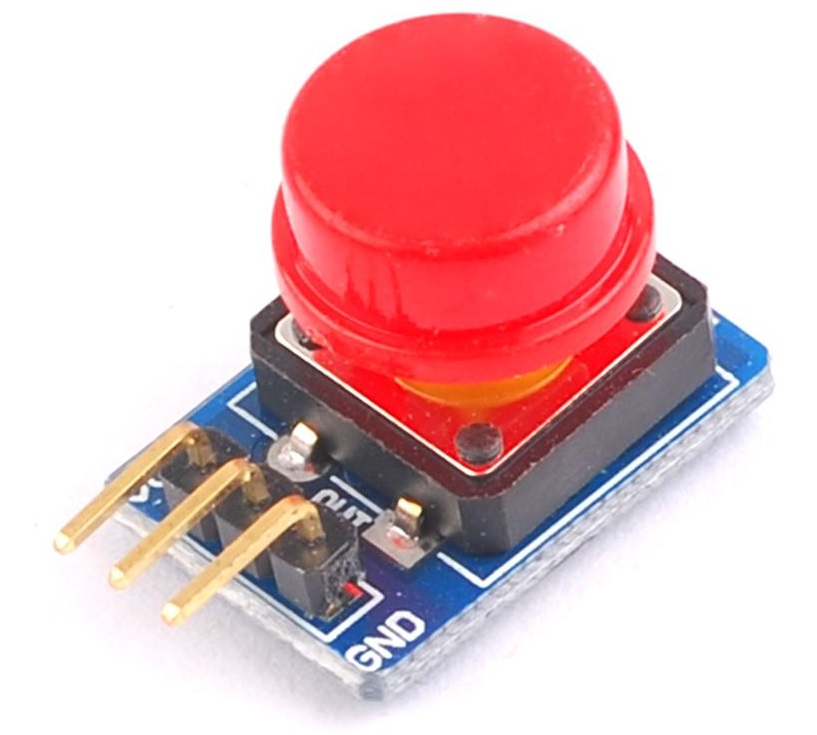
\includegraphics[width=2.5cm]{pictures/button.png} \\
    \hline
\end{tabular}
\end{center}
\cleardoublepage
\textbf{Mô tả chức năng các linh kiện chính}
\begin{itemize}
    \item \textbf{PIC16F887}: Vi điều khiển chính điều khiển toàn bộ hoạt động của hệ thống, bao gồm xử lý chế độ, điều khiển đèn, hiển thị và đọc nút nhấn.
    \item \textbf{Đế ra chân PIC}: Dùng để cố định và kết nối PIC16F887 với breadboard hoặc mạch in, thuận tiện cho lắp ráp và tháo rời.
    \item \textbf{Mạch đèn giao thông}: Gồm 3 LED (đỏ, vàng, xanh) mô phỏng các tín hiệu giao thông ở ngã tư.
    \item \textbf{Module 2 LED 7 đoạn 74HC595}: Hiển thị thời gian đếm ngược trong từng pha đèn, được điều khiển thông qua IC dịch 74HC595 nhằm giảm số lượng chân I/O của vi điều khiển.
    \item \textbf{LCD 1602}: Hiển thị chế độ hoạt động của hệ thống (AUTO, MANUAL, NIGHT), giúp người dùng dễ dàng theo dõi trạng thái.
    \item \textbf{Module I2C giao tiếp LCD}: Cho phép kết nối LCD với vi điều khiển qua giao tiếp I2C, giảm số lượng chân cần dùng.
    \item \textbf{Nút nhấn}: Dùng để chuyển đổi chế độ hoạt động và điều khiển pha đèn trong chế độ thủ công.
\end{itemize}
\cleardoublepage